\documentclass[journal]{vgtc}                % final (journal style)
%\documentclass[review,journal]{vgtc}         % review (journal style)
%\documentclass[widereview]{vgtc}             % wide-spaced review
%\documentclass[preprint,journal]{vgtc}       % preprint (journal style)

%% Uncomment one of the lines above depending on where your paper is
%% in the conference process. ``review'' and ``widereview'' are for review
%% submission, ``preprint'' is for pre-publication, and the final version
%% doesn't use a specific qualifier.

%% These few lines make a distinction between latex and pdflatex calls and they
%% bring in essential packages for graphics and font handling.
%% Note that due to the \DeclareGraphicsExtensions{} call it is no longer necessary
%% to provide the the path and extension of a graphics file:
%% 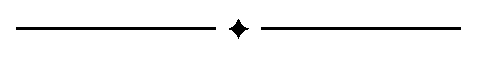
\includegraphics{diamondrule} is completely sufficient.
%%
\ifpdf%                                % if we use pdflatex
  \pdfoutput=1\relax                   % create PDFs from pdfLaTeX
  \pdfcompresslevel=9                  % PDF Compression
  \pdfoptionpdfminorversion=7          % create PDF 1.7
  \ExecuteOptions{pdftex}
  \usepackage{graphicx}                % allow us to embed graphics files
  \DeclareGraphicsExtensions{.pdf,.png,.jpg,.jpeg} % for pdflatex we expect .pdf, .png, or .jpg files
\else%                                 % else we use pure latex
  \ExecuteOptions{dvips}
  \usepackage{graphicx}                % allow us to embed graphics files
  \DeclareGraphicsExtensions{.eps}     % for pure latex we expect eps files
\fi%

%% it is recomended to use ``\autoref{sec:bla}'' instead of ``Fig.~\ref{sec:bla}''
\graphicspath{{figures/}{pictures/}{images/}{./}} % where to search for the images

\usepackage{microtype}                 % use micro-typography (slightly more compact, better to read)
\PassOptionsToPackage{warn}{textcomp}  % to address font issues with \textrightarrow
\usepackage{textcomp}                  % use better special symbols
\usepackage{mathptmx}                  % use matching math font
\usepackage{times}                     % we use Times as the main font
\renewcommand*\ttdefault{txtt}         % a nicer typewriter font
\usepackage{cite}

% added by Connor
\usepackage{subfig}
\usepackage{balance}

%% If you are submitting a paper to a conference for review with a double
%% blind reviewing process, please replace the value ``0'' below with your
%% OnlineID. Otherwise, you may safely leave it at ``0''.
\onlineid{0}

%% declare the category of your paper, only shown in review mode
\vgtccategory{Research}

%% Paper title - 1 pt for descriptive title
\title{Analysis of Execution Trace Lines in Gantt Charts}

%% This is how authors are specified in the journal style

%% indicate IEEE Member or Student Member in form indicated below
%% 1 pt for name
\author{Connor Scully-Allison}
\authorfooter{
%% insert punctuation at end of each item
\item
 Connor Scully-Allison is a graduate student at the University of Arizona. E-mail: cscully-allison@email.arizona.edu.
}

%other entries to be set up for journal
%\shortauthortitle{Firstauthor \MakeLowercase{\textit{et al.}}: Paper Title}

%% Abstract section - 5 pts
\abstract{
In the HPC domain, a problem that plagues execution trace visualizations is an inability to meaningfully render communications on Gantt charts for modern supercomputers. The number of concurrent processors being monitored makes it impossible to draw all communication connections at once. This is problematic as understanding communication between processes is crucial to optimizing programs which use these HPC resources and must be as performant as possible. To better understand this problem we propose a within-subjects study designed to evaluate what repeated marks may be necessary and which may be redundant in displaying commonly found HPC communication patterns. This experiment will be piloted and iterated on until it is ready to be deployed to a large base of users so that meaningful data can be collected. Data collected from this experiment can help inform a design study which will produce a better Gantt chart. One that can represent communications data at scale.

} % end of abstract

%% Keywords that describe your work. Will show as 'Index Terms' in journal
%% please capitalize first letter and insert punctuation after last keyword
%\keywords{Radiosity, global illumination, constant time}

%% ACM Computing Classification System (CCS). 
%% See <http://www.acm.org/class/1998/> for details.
%% The ``\CCScat'' command takes four arguments.

%\CCScatlist{ % not used in journal version
% \CCScat{K.6.1}{Management of Computing and Information Systems}%
%{Project and People Management}{Life Cycle};
% \CCScat{K.7.m}{The Computing Profession}{Miscellaneous}{Ethics}
%}

%% Uncomment below to include a teaser figure.
%   \teaser{
%   \centering
%   \includegraphics[width=16cm]{CypressView}
%   \caption{In the Clouds: Vancouver from Cypress Mountain.}
%  }

%% Uncomment below to disable the manuscript note
%\renewcommand{\manuscriptnotetxt}{}

%% Copyright space is enabled by default as required by guidelines.
%% It is disabled by the 'review' option or via the following command:
% \nocopyrightspace

\vgtcinsertpkg

%%%%%%%%%%%%%%%%%%%%%%%%%%%%%%%%%%%%%%%%%%%%%%%%%%%%%%%%%%%%%%%%
%%%%%%%%%%%%%%%%%%%%%% START OF THE PAPER %%%%%%%%%%%%%%%%%%%%%%
%%%%%%%%%%%%%%%%%%%%%%%%%%%%%%%%%%%%%%%%%%%%%%%%%%%%%%%%%%%%%%%%%

\begin{document}

%% The ``\maketitle'' command must be the first command after the
%% ``\begin{document}'' command. It prepares and prints the title block.

%% the only exception to this rule is the \firstsection command
\firstsection{Introduction} % or "Motivation"

\maketitle

% Introduction and/or Motivation - 15 pts

Strongly motivate your project in this section.

Summarize the problem you are trying to solve.

Explain why the problem is important -- who benefits from the problem being
solved and in what way? If the problem were to be solved, what would that
enable people to do?

Summarize what you plan to do to solve the problem.

% You may want to end this section by summarizing it again as a list:
The aims of this research are:
\begin{itemize}
  \item a taxonomy of tasks performed in the visual analysis of octopi 
  \item a validated visual design supporting the visual analysis of octopi
\end{itemize}

 

% 10 pts
\section{Background}
\label{sec:background}

This research applies significantly to high performance computing (HPC), so to understand it some understanding of HPC concepts are necessary. First is the concept of profiling. Profiling generally describes the process of measuring a program's execution using various metrics like runtime and memory usage. This information is used to optimize a program and is crucial to understanding the complex and large programs developed to run on distributed systems and supercomputers.

When profiling parallel programs there are many characteristics which experts examine. Among them, communication between processes is one of the most important. This communication is often abstracted as "messages" passed between programs conveying state information or containing data. Because supercomputers commonly do not share memory this data must be transferred between CPU's using physical buses or network connections. The most common library used for this process is called "Message Passing Interface" or MPI. The time taken to transfer this data is called "overhead" and describes a common phenomenon that causes slowdown with parallel programs.


A Gantt chart describes a special variety of chart which plots tasks along a timeline with bars. The x axis commonly denotes time in these charts and the y axis usually denotes a category. In HPC, each bar denotes a particular process or processor running a portion of parallel code. This bar can be subdivided into sections that denote function calls or execution states. Straight lines indicate passed messages between processes and connect bars at various points. An example of a typical Gantt chart can be seen in Figure \ref{fig:simple_gantt}.


% 5 pts
\subsection{Related Work}
\label{sec:related}
Gantt charts have been used as a key visualization method in HPC profiling software for many years. Introduced as a "timeline" view by VAMPIR in 1996, many other platforms adapted the design they presented to visualize execution traces \cite{nagel1996vampir}.  Notably, Intel provides a "Intel Trace Analyzer" software which uses a nearly identical layout to VAMPIR\cite{Intel2019}. HPCToolkit similarly provides a Gantt chart view tracing the execution of various processes over time, however they omit the lines denoting message passing between processes\cite{Adhianto2009}.

As is implied by HPCToolkit, the use of connecting lines to denote passed messages is not universal. However it can provide critical contextual information which aids researchers looking for bottlenecks. This approach was notably introduced as a means to give programmers insight into the structure of communication between threads and cores\cite{Leblanc1990}. At small scales this insight can be highly informative as to how communication overhead may impact the efficiency of parallel programs. 

The concept of developing a Gantt chart for the modern era of HPC is not a new one. Acknowledging the failure of traditional techniques for HPC profiling and visualization, there has been continual effort to improve the general layout of Gantt charts to provide more meaningful information \cite{Cottam2015, Adhianto2016HPCToolkit, Tallent2011}. Although impactful, much of this work is generally focused on an improvement of scaling process bars in timelines and coding more information into those bars. 

More specific to the subject of this paper, there does exist some work which attempts to preserve the message passing information encoded with lines at modern scales. Researchers in Germany have attempted integrate a commonly found graph visualization technique called "edge bundling" into Gantt charts to reduce visual clutter of these connecting lines \cite{Brendel2016}. There has also been research which seeks to mitigate noise caused by unnecessary edge crossings in physical timelines by converting them to logical time\cite{isaacs2014combing}. These approaches have had success in simplifying visualizations but can still obscure other information in their charts and suffer from scaling issues as more and more processes are added. 

Despite being widely used in HPC profiling, there exists very little work evaluating Gantt charts' effectiveness with empirical, user-study based research. The closest work in recent years, which provides a good model for this sort of evaluation comes from Sambasivan et al \cite{Sambasivan2013}. This work on request flow comparisons provides us with some insight into how best to design a study in this domain and some metrics to consider for evaluation.



\section{Research Plan} 
\label{sec:research}

% 30 pts for explanation here combined with timeline below
Re-state the problem you are trying to solve and then explain how you plan to
solve it. Is it designing a new visualization? Is it designing a new library?
Is it running a controlled experiment? Is it something else?

Note this is a {\em plan}. The plan may change as you make discoveries during
your project. However, you must describe what your plan is assuming everything
goes as expected. If there are some parts of the plan where you could run into
difficulties, state what those difficulties are and what alternative measures
you could take should those difficulties arise.

You may refer to other sections so as not to repeat yourself -- for example,
referencing Section~\ref{sec:background}.

You may want to use figures to illustrate your point, such as
Figure~\ref{fig:sample}.

\begin{figure}[h]
 \centering % avoid the use of \begin{center}...\end{center} and use \centering instead (more compact)
 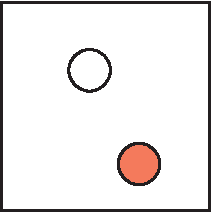
\includegraphics[width=1.5in]{figs/sample}
 \caption{Figure illustrating some proposed designs.}
 \label{fig:sample}
\end{figure}

% 5 pts
\subsection{Data}
\label{sec:data}

Describe the data here. Describe whether you already have access to the data
and if not, what is required to obtain the data. If you don't already have the
data, explain how long it will take to retrieve it. 

% 15 pts
\subsection{Evaluation}
\label{sec:eval}

Describe your plan for evaluating your work during this project.

Then, describe how you would evaluate the work beyond the timeframe of the
project. Without time constraints, what would you do? Do you have the
resources (people, time, equipment, data, money) to implement this plan in
the future? Does your plan for evaluating your work during the project serve
as a first step to this evaluation?

% 5 pts
\subsection{Technology}
\label{sec:tech}

Describe what technologies you intend to use (e.g., programming languages,
platforms, existing libraries) and why they make sense for your project. Do
they serve your users better than other technologies? Are you able to take
advantage of existing work/libraries for your domain with this technology
rather than HTML/CSS/JS and d3js?  

\subsection{Timeline}
\label{sec:timeline}

Adapt the milestones for the class project to the specifics of your project
and summarize in Table~\ref{tab:milestones}. Do not simply copy the current
text as is. Your milestones should be specific to your problem.

The expectations are as follows:

\vspace{1.5ex}\noindent\textbf{Project Milestone Two} should include any task
and data abstraction necessary to support the project design whether it is
designing a user study, designing a new visualization, or designing a new
library. Initial designs should be included with discussion of the rationale
in support of the design. Data supporting all of these findings in terms of
background work or newly collected data (e.g., interviews, observations)
should be cited or discussed.

Additionally, the related works should be updated with a more thorough
literature review. Changes to the status of the data and the choices of
technology should be discussed.

If you are doing a literature review or a taxonomy, you should have a
preliminary list of papers you will review, along with an explanation of the
methodology you used to generate that list of papers (e.g., which venues did
you start with? which years? how did you follow citations?)

\vspace{1.5ex}\noindent\textbf{Project Milestone Three} should include the
results of the first chunk of work that needs to be done. In most projects
with implementation this will involve a working data reader and at least one visualization,
library feature, or study question type working. The milestone should include
images of these features and a discussion of what they do. The demonstration
should run with minimal effort and the code should be included in the
repository. For projects involving heavy literature review, this milestone
should include annotations and notes for half of the selected papers.
Including a preliminary schema will help me give you feedback.

In the corresponding report, discussion of project progress as well as any
revisions to the data, technology choice, and scope should be included.

\vspace{1.5ex}\noindent\textbf{Project Milestone Four} should include a
complete working prototype of the main project artifact, such as a
visualization tool, a visualization library, a working study with experimental
objects and stimuli complete, or completed literature annotations with an
categorization schema. The demonstration should run with minimal effort and
the code should be included in the repository.

In the corresponding report, discussion of project progress as well as any
revisions to the data, technology choice, and scope should be included. The
plan for evaluation especially should be updated indicating the plan for
milestone five and any preliminary work in the design of that evaluation.


\vspace{1.5ex}\noindent\textbf{Project Milestone Five} should include initial
evaluation of the work from project milestone four and recommendations for
improvement. Artifacts generated (e.g., pre-observation
plan, observation notes, data from studies) during this evaluation should be
included in the repository. Literature-based projects should include a
refinement of the findings from the previous milestone.

Additionally, a full report of the project as a whole should be included in
this milestone.



\begin{table}[h]
%% Table captions on top in journal version
 \caption{Project Milestones}\vspace{1ex} % the \vspace adds some space after the top caption
 \label{tab:milestones}
 \scriptsize
 \centering % avoid the use of \begin{center}...\end{center} and use \centering instead (more compact)
   \begin{tabular}{r|r}
     Milestone & Description (\%)\\
   \hline
     PM2 & Conduct interviews with hydrologists, sketch designs, \\
         & data and task abstractions written\\
     PM3 & Central (map) view of data working with basic pan and \\
         & zoom interactions, initial structure for multiple \\
	 & coordinated view\\
     PM4 & All views working including histogram selector and list \\
	 & view, advanced interactions added to map view, preliminary \\
	 & tasks selected for evaluation \\
     PM5 & Evaluation sessions with three hydrologists, data coded \\
         & and summarized.\\
   \end{tabular}
\end{table}



% 10 pts
\section{Impacts}
\label{sec:impact}

The primary impact of this research is quantifying how people derive meaningful information from marks of lines and patterns of lines, specifically in the context of tracing communication in parallel programs. Even if the data obtained from this experiment supports common sense expectations, this work can then be used to justify design decisions made by future iterations of existing Gantt chart visualization software.

More concretely, the conclusions drawn from this work can be leveraged to inform a guided design study with the goal of building a better Gantt chart that effectively visualizes communication at large scales. Innovation on this front can significantly impact contemporary profiling workflows with large, distributed supercomputer clusters. If future profiling visualization software can show these communication patterns using more succinct notation, domain professionals will be able to locate bottlenecks significantly faster than current software allows for.



%\bibliographystyle{abbrv}
\bibliographystyle{abbrv-doi-hyperref}
%%use following if all content of bibtex file should be shown
%\nocite{*}
\balance
\bibliography{proposal}
\end{document}

